\documentclass[12pt]{article}
\usepackage{mathtools}
\usepackage{amssymb}
\usepackage{amsthm}
\usepackage{pgfplots}
\usepackage{tikz}
\usetikzlibrary{calc}
\usepackage{polski}
\usepackage[utf8]{inputenc}
\usepackage{geometry}
\usepackage{amsmath}
\usepackage{mnsymbol}
\usepackage{graphicx}
\usepackage{textgreek}
\usepackage{float}
\usepackage{caption}
\begin{document}
\newgeometry{tmargin=2cm,bmargin=2cm,lmargin=2cm,rmargin=2cm}
\tableofcontents \newpage
\section{Cel ćwiczenia}
Celem ćwiczenia było wyznaczenie modułu Younga metodą statyczną polegającą na zmierzeniu wydłużenia drutu z badanego metalu obciążonego stałą siłą.
\section{Wstęp teorytyczny}
\noindent Nie w każdym przypadku możemy posługiwać się pojęciem bryły sztywnej. Wiele rzeczywistych ciał zmienia swój kształt pod wpływem przyłożonych do nich sił. 
Jeżeli po usunięciu tych sił ciało wraca do pierwotnego kształtu, mamy wówczas do czynienia z odkształceniem sprężystym. Związane z tym terminem prawo 
Hooke'a mówi, że odształcenie sprężyste ciała jest proporcjonalne do przyłożonej do niego siły. Prawo to jest prawdziwe dla dowolnego kształtu ciała i konfiguracji 
przyłożonych sił. Dla przypadku rozciągania jednorodnego pręta (widocznego na Rys. 1), przyrost długości pręta $\Delta{l}$ jest proporcjonalny do jego długości 
$l$ oraz siły $F$, a odwrotnie proporcjonalny do przekroju poprzecznego $S$. Przyrost długości możemy wówczas wyrazić: 
\begin{center}
\LARGE $ \Delta{l} = \frac{F l}{E S} $,
\end{center}
gdzie stała materiałowa E nazywana jest modułem Younga. Jednostką modułu Younga jest Paskal. 
\begin{figure}[H]
\centering
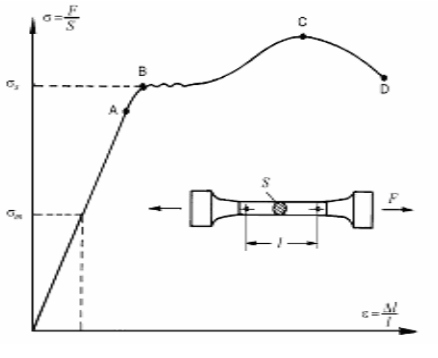
\includegraphics[width=10cm]{1}
\caption*{\textbf{Rys. 1}: Charakterystyka rozciągania typowa dla większości metali. A - granica proporcjonalności, B - granica sprężystości, 
C - punkt maksymalnego naprężenia, D - punkt zerwania}
\end{figure} \noindent
Naprężeniem nazywamy miarę gęstości powierzchniowej sił wewnętrznych. Miarą naprężenia jest Paskal. Zwykle rozkładamy naprężenie na dwie składowe: naprężenie normalne prostopadłe do płaszczyzny powierzchni przekroju i naprężenie styczne działające w płaszczyźnie powierzchni przekroju.
W zależności od sposobu przyłożenia sił zewnętrznych mamy następujące przypadki obciążeń: rozciąganie lub ściskanie, zginanie, skręcanie. \newpage \noindent
W przypadku rozciągania (ściskania) pręta prawo Hooke'a możemy wyrazić wzorem:
\begin{center}
\LARGE $ \sigma = E \varepsilon $,
\end{center}
gdzie $\sigma$ to naprężenie normalne zaś $\varepsilon$ to normalne odkształcenie względne. Naprężenie normalne definiujemy jako stosunek przyłożonej siły
do pola przekroju pręta $\sigma = \frac{F}{S}$ zaś normalne odkształcenie względne to stosunek przyrostu długości pręta do jego długości początkowej 
$ \varepsilon = \frac{\Delta{l}}{l}$. 
Podana zależność charakteryzuje stan naprężeń i odkształceń w rozciąganej (ściskanej) próbce niezależnie od kształtu próbki. \newline
Hipotetycznie wartość modułu Younga to naprężenie, które wystąpiłoby przy dwukrotnym wydłużeniu próbki materiału, przy założeniu, że jej przekrój nie zmieni się.
	W rzeczywistości w większości przypadków prawo Hooke'a przestaje obowiązywać znacznie wcześniej więc napisana wyżej definicja nie sprawdza się. Rysunek 1 przedstawia cztery charakterystyczne punkty zależności naprężenie - odkształcenie typowej dla większości metali. Pierwszym z nich jest granica proporcjonalności, na której kończy się odcinek liniowy wykresu. Drugim jest granica sprężystości, po przekroczeniu której zaczyna się nieodwracalne odkształcenie materiału. Trzecim punktem jest punkt maksymalnego naprężenia, zaś ostatnim punkt, w którym materiał ulega zerwaniu. W przypadku materiałów kruchych materiał po osiągnięciu granicznego naprężenia pęka. \newline
Doświadczenie polegało na bezpośrednim pomiarze wielkości wchodzących w skład wzoru $ \Delta{l} = \frac{F l}{E S} $ przy pomocy przyrządzów opisanych w punkcie 3, zaś sposób mierzenia danych wielkości opisany został w punkcie 4. Podczas wykonywania ćwiczenia należało pamiętać, że pręt i szalka zamocowane są w połowie odległości między osią obrotu a punktem styku z czujnikiem mikrometrycznym, co skutkuje tym, że zmierzone wydłużenie drutu $\Delta{l}$ jest dwa razy większe niż w rzeczywistości.\newline W naszym doświadczeniu siłą $F$ rozciągającą drut była siła ciężkości odważników na szalce o łącznej masie $m$. Siła ta wyraża się zatem wzorem $F = mg$, gdzie $g$ to przyspieszenie ziemskie. Prawo Hooke'a mówi nam, że zależność $\Delta{l}(F)$ powinna być linią prostą a zatem porównanie współczynnika $a$ z równania $ \Delta{l} = aF + b$ z wzorem wyrażającym prawo Hooke'a daje nam możliwość obliczenia wartości modułu Younga. Po odpowiednich przekształceniach dostajemy $E = \frac{l}{aS}$. Dodając do tego fakt, że pole przekroju druta S możemy wyrazić wzorem $S = \frac{\pi{d^2}}{4}$, otrzymujemy roboczy wzór na moduł Younga:
\begin{center}
\LARGE $ E = \frac{4l}{\pi{d^2}a} $,
\end{center}
Względną niepewność złożoną $u_c(E)$ można obliczyć przy pomocy prawa propagacji niepewności względnej na podstawie wcześniej oszacowanych niepewności $l$,$d$ oraz $a$. Wyraża się ona wzorem:
\begin{center}
\LARGE $ \frac{u_c(E)}{E} = \sqrt{(\frac{u(l)}{l})^2+(-2\frac{u(d)}{d})^2+(-\frac{u(a)}{a})^2} $,
\end{center} \newpage
\section{Układ pomiarowy} 
Przyrządy potrzebne do wykonania doświadczenia: \newline
1. Przyrząd do pomiaru wydłużenia drutu pod wpływem stałej siły (Rys. 2), zaopatrzony w czujnik mikrometryczny do pomiaru wydłużenia drutu. \newline
2. Zestaw odważników. \newline
3. Śruba mikrometryczna \newline
4. Przymiar milimetrowy \newline
5. Kalkulator \newline
\begin{figure}[H]
\centering
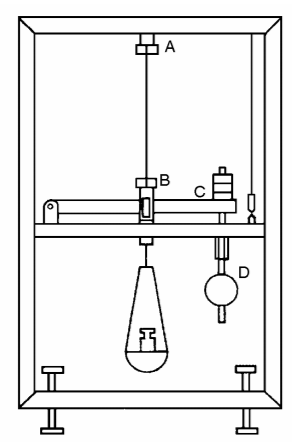
\includegraphics[width=6cm]{2}
\caption*{\textbf{Rys. 2}: Urządzenie do pomiaru modułu Younga metodą statyczną }
\end{figure}
\section{Przebieg ćwiczenia}
Aby poprawnie wykonać doświadczenie najpierw należało zmierzyć długość $l$ drutu, który został użyty do wyznaczenia modułu Younga. Następnie niezbędne było zamocowanie drutu w statywie za pomocą nakrętek i obciążenie szalki dwoma jednokilogramowymi odważnikami oraz zmierzenie za pomocą śruby mikrometrycznej średnicy drutu w trzech różnych miejscach rozłożonych na całej jego długości. Po opróżnieniu szalki z odważników należało zwolnić blokadę belki pomiarowej, a następnie wyregulować zamocowanie drutu tak, aby belka dotykała końcówki czujnika mikrometrycznego. W dalszej kolejności należało wyzerować wskazania czujnika mikrometrycznego. Po naciśnięciu ręką na szalkę i sprawdzeniu czy czujnik mikrometryczny reaguje i czy wraca w położenie zerowe, należało obciążać szalkę przez dokładanie kolejnych odważników, jednocześnie notując w tabeli sumaryczną masę odważników i wynikające wydłużenie drutu. Konieczne było wykonanie pomiarów dla rosnących a następnie dla malejących wartości ciężaru. Po zakończeniu, ćwiczenie powtórzyliśmy dla drutu wykonanego z innego metalu. 
\section{Wyniki pomiarów}
\begin{figure}[H]
\centering
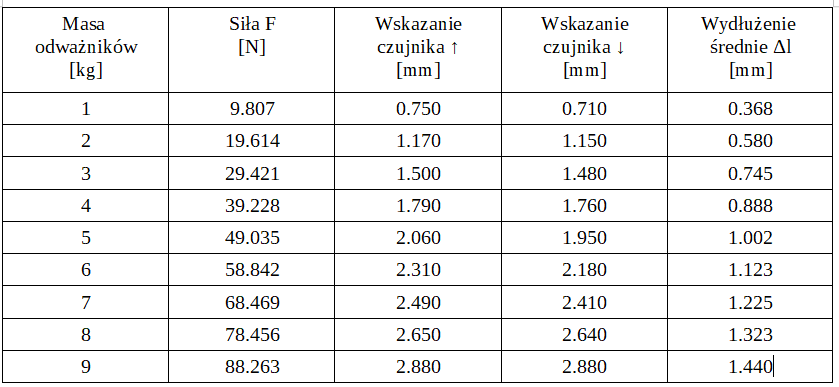
\includegraphics[width=18cm]{3}
\caption*{\textbf{Tab. 1}: Tabela z wynikami pomiarów dla stalowego drutu. Zmierzona długość drutu l to \newline $107.0$ $cm$. Jako jej niepewność przyjęliśmy działkę elementarną $u(l)=0.1$ $cm$}
\end{figure}
\begin{figure}[H]
\centering
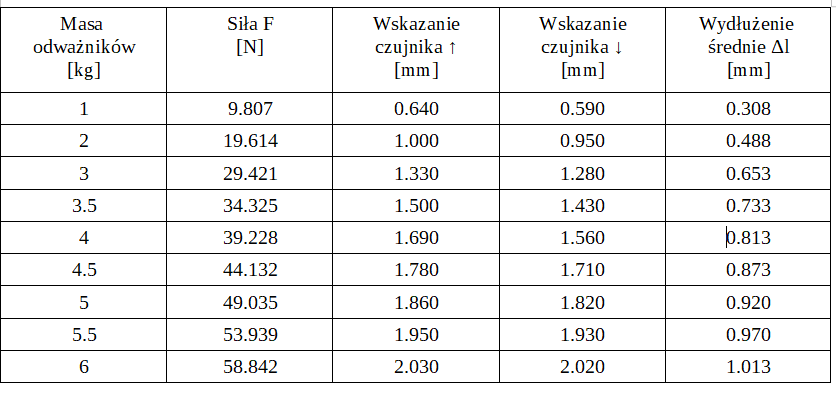
\includegraphics[width=18cm]{4}
\caption*{\textbf{Tab. 2}: Tabela z wynikami pomiarów dla mosiężnego drutu. Zmierzona długość drutu l to \newline $107.3$ $cm$. Jako jej niepewność przyjęliśmy działkę elementarną $u(l)=0.1$ $cm$ }
\end{figure}
\section{Opracowanie wyników pomiaru}
\subsection{Wartość średnia średnicy drutu}
W doświadczeniu zmierzyliśmy przy pomocy śruby mikrometrycznej średnice drutu w trzech różnych miejscach. Dla drutu stalowego te pomiary wyniosły $0.80$ $mm$, $0.81$ $mm$, $0.80$ $mm$ , zaś dla drutu mosiężnego $1.20$ $mm$, $1.20$ $mm$, $1.20$ $mm$. Zatem wartością średnią średnicy drutu jest średnia arytmetyczna wszystkich wyników. Dla drutu stalowego średnica średnia wynosi $0.80$ $mm$ , zaś dla drutu mosiężnego $1.20$ $mm$. Niepewność wartości średniej średnicy drutu wyznaczyliśmy przy pomocy metody typu B (na podstawie działki elementarnej przyrządu) i wyniosła ona \newline $u(d)=0.01$ $mm$.
\subsection{Wykres zależności średniego wydłużenia drutu $\Delta{l}$ w funkcji przyłożonej siły rozciągającej $F$}
\begin{center}
\begin{tikzpicture}[scale=1.5]
\begin{axis}[
title={Drut stalowy},
xlabel={Wartość przyłożonej siły rozciągającej $F [N]$},
ylabel={Średnie wydłużenie $\Delta{l}$ drutu$[mm]$},
xmin=9,xmax=90,
ymin=0.3,ymax=1.5,
legend pos=north west,
ymajorgrids=true,grid style=dashed
]

\addplot[color=black,mark=square, only marks]
coordinates {
(9.807,0.368)
(19.614,0.580)
(29.421,0.745)
(39.228,0.888)
(49.035,1.002)
(58.842,1.123)
(68.469,1.225)
(78.456,1.323)
(88.263,1.440)
};

\end{axis}
\end{tikzpicture} \newpage
\begin{tikzpicture}[scale=1.5]
\begin{axis}[
title={Drut mosiężny},
xlabel={Wartość przyłożonej siły rozciągającej $F [N]$},
ylabel={Średnie wydłużenie $\Delta{l}$ drutu $[mm]$},
xmin=9,xmax=60,
ymin=0.3,ymax=1.1,
legend pos=north west,
ymajorgrids=true,grid style=dashed
]

\addplot[color=black,mark=square, only marks]
coordinates {
(9.807,0.308)
(19.614,0.488)
(29.421,0.653)
(34.325,0.733)
(39.228,0.813)
(44.132,0.873)
(49.035,0.920)
(53.939,0.970)
(58.842,1.013)
};

\end{axis}
\end{tikzpicture}
\end{center}
\subsection{Dopasowanie prostej metodą najmniejszych kwadratów}
Do znalezienia prostej liniowej dopasowanej do wykresu użyliśmy regresji liniowej. Wspomogliśmy się arkuszem kalkulacyjnym, który wyznaczył nam linię dopasowania. Dla stalowego drutu:
\begin{center}
\LARGE $ \Delta{l} = 0.01311\frac{mm}{N}\;F+0.323\frac{mm}{N} $
\end{center}
Program wyznaczył również niepewności pomiarowe $ u(a) = 0.00062 $ $mm/N $ oraz \newline $ u(b) = 0.034$ $mm/N $. \newline
Dla mosiężnego drutu została znaleziona linia:
\begin{center}
\LARGE $ \Delta{l} = 0.01445\frac{mm}{N}\;F+0.209\frac{mm}{N} $
\end{center}
Program wyznaczył również niepewności pomiarowe $ u(a) = 0.00072 $ $mm/N $ oraz \newline $ u(b) = 0.029 $ $mm/N $. \newline
\begin{center}
\begin{tikzpicture}[scale=1.5]
\begin{axis}[
title={Drut stalowy},
xlabel={Wartość przyłożonej siły rozciągającej $F [N]$},
ylabel={Średnie wydłużenie $\Delta{l}$ drutu$[mm]$},
legend pos=north west,
ymajorgrids=true,grid style=dashed
]

\addplot[color=black,mark=square, only marks]
coordinates {
(9.807,0.368)
(19.614,0.580)
(29.421,0.745)
(39.228,0.888)
(49.035,1.002)
(58.842,1.123)
(68.469,1.225)
(78.456,1.323)
(88.263,1.440)
};

\addplot [
	domain=9:90,
	samples=100,
	color=red,
] 
{0.013114187*x+0.323208121};
\end{axis}
\end{tikzpicture} \newline
\begin{tikzpicture}[scale=1.5]
\begin{axis}[
title={Drut mosiężny},
xlabel={Wartość przyłożonej siły rozciągającej $F [N]$},
ylabel={Średnie wydłużenie $\Delta{l}$ drutu $[mm]$},
legend pos=north west,
ymajorgrids=true,grid style=dashed
]

\addplot[color=black,mark=square,only marks]
coordinates {
(9.807,0.308)
(19.614,0.488)
(29.421,0.653)
(34.325,0.733)
(39.228,0.813)
(44.132,0.873)
(49.035,0.920)
(53.939,0.970)
(58.842,1.013)
};
\addplot [
	domain=9:60,
	samples=100,
	color=red,
] 
{0.014448566*x+0.209158759};
\end{axis}
\end{tikzpicture}
\end{center}
\subsection{Obliczenie modułu Younga}
Zgodnie z prawem Hooke'a zależność  $\Delta{l}(F)$ powinna być linią prostą. Porównanie równania prostej $\Delta{l} = aF + b$ z wzorem $\Delta{l}=\frac{Fl}{ES}$ pozwala nam utożsamić współczynnik $a$ z czynnikiem $\frac{l}{ES}$, zatem $E=\frac{l}{aS}$. Biorąc pod uwagę również fakt, że pole przekroju drutu $S$
obliczamy ze średnicy $d$ jako $S=\frac{\pi{d^2}}{4}$, nasz roboczy wzór na moduł Younga przyjmuje postać:
\begin{center}
\LARGE $E=\frac{4l}{\pi{d^2}a}$
\end{center}
Dla stalowego drutu:
\begin{center}
\LARGE $E_{stal}=\frac{4*1070\;mm}{\pi*(0.80\;mm)^2*0.013114187 \;\frac{mm}{N}} = 162300\;\frac{N}{mm^2} = 162.3\;GPa $
\end{center}
Dla mosiężnego drutu:
\begin{center}
\LARGE $E_{mos}=\frac{4*1073\;mm}{\pi*(1.20\;mm)^2*0.014448566 \;\frac{mm}{N}} = 65700\;\frac{N}{mm^2} = 65.7\;GPa $
\end{center}
\subsection{Obliczenie niepewności wartości $E$ wykorzystując prawo \newline propagacji niepewności względnej}
Niepewność złożoną $u_c(E)$ możemy obliczyć przy pomocy prawa propagacji niepewności względnej na podstawie niepewności $l$,$d$ oraz $a$. Zakładamy, że niepewność masy $m$ jest pomijalnie mała. Wzór przyjmuje postać:
\begin{center}
\LARGE $\frac{u_c(E)}{E} = \sqrt{(\frac{u(l)}{l})^2+(-2\frac{u(d)}{d})^2+(-\frac{u(a)}{a})^2}$
\end{center}
Dla stalowego drutu:
\begin{center}
\Large $u_c(E_{stal}) = 162.3\;GPa * \sqrt{(\frac{1\;mm}{1070\;mm})^2+(-2\frac{0.01\;mm}{0.80\;mm})^2+(-\frac{0.000618638\;\frac{N}{mm^2}}{0.013114187\;\frac{N}{mm^2}})^2} = 8.7\;GPa$
\end{center}
Dla mosiężnego drutu:
\begin{center}
\Large $u_c(E_{mos}) = 65.7\;GPa * \sqrt{(\frac{1\;mm}{1073\;mm})^2+(-2\frac{0.01\;mm}{1.20\;mm})^2+(-\frac{0.00072181\;\frac{N}{mm^2}}{0.014448566\;\frac{N}{mm^2}})^2} = 3.5\;GPa$
\end{center} 
\subsection{Niepewność rozszerzona $U_c(E)$}
Przyjmując poziom ufności k = 2, obliczyliśmy niepewność rozszerzoną $U_c(E)$ korzystając ze wzoru:
\begin{center}
\LARGE $ U_c(E) = k * u_c(E)  $
\end{center}
Wartości $U_c(E)$ dla stalowego i mosiężnego drutu to odpowiednio $17.4\;GPa$ oraz $7.0\;GPa$.
\section{Wnioski}
Zmierzona wartość modułu Younga dla stalowego drutu wynosi $162.3\;GPa$ z niepewnością rozszerzoną $8.7\;GPa$, zaś dla mosiężnego drutu $65.7\;GPa$ z niepewnością rozszerzoną $3.5\;GPa$. Wartości tablicowe dla stali i mosiądzu, według opisu ćwiczenia, to odpowiednio $210-220\;GPa$,$100\;GPa$. Otrzymane wartości znacznie różnią się od tabelarycznych, nawet po uwzględnieniu niepewności rozszerzonych. Najprawdopodobniej spowodowane jest to wieloma czynnikami takimi jak zmęczenie drutów, niedokładność pomiarów długości drutu oraz jego średnicy, którą bardzo trudno jest dokładnie zmierzyć. Ważnym czynnikiem również był fakt, że używane druty nie były wystarczająco proste. Zarówno drut stalowy jak i mosiężny początkowo prostowały się zamiast rozciągać. Skutkowało to mniejszymi wartościami $\Delta{l}$, te zaś skutkowały większym współczynnikiem nachylenia prostej $a$, który zaniżał wartość modułu Younga $E$. Wynika z tego, że dla pomiarów warto odrzucić początkowe punkty pomiarowe, ponieważ wtedy drut dopiero się prostuje.
\end{document}
